%==============================================================================
\section{Introduction}
\label{sec:introduction}
%==============================================================================

Causal Loop Diagrams (CLDs) are qualitative representations of hypothesized causal structure---directed graphs where nodes represent variables and signed edges represent positive or negative causal influences---that serve as precursors to computational models, enabling intervention simulations and informing new theories and experiments. However, CLD construction cost scales as $O(|V|^2)$ for a system with $|V|$ variables, making large-variable systems prohibitively expensive to create---especially through group model-building sessions where expert time is scarce and coordination is challenging (Figure~\ref{fig:expert_review_burden_llm_assisted}). This thesis focuses on health-domain CLDs---specifically models of obesity, Alzheimer's disease, and emergency department visits---where causal modeling directly informs clinical decision-making and intervention design.

\medskip
\noindent
\textbf{The information aggregation challenge.} The rapid increase in research output brings opportunities for knowledge synthesis and subsequent new knowledge creation, but also significant challenges in efficiently aggregating this information. This aggregation step is crucial to presenting a complete perspective in which interactions between variables are accounted for---a key factor in understanding complex biological systems in the clinic, in research, and for constructing computational models. However, individual researchers cannot keep up with new research given the exponentially increasing volume of publications and the fundamental limits of knowledge accumulation feasible for a single person.

To address this limitation and aggregate siloed knowledge, domain expert sessions can be used to exchange and compile specialized knowledge into a single causal loop diagram, which can then be converted into a computational model for use in research, diagnosis, and intervention simulation. However, since expert time is scarce, these sessions are difficult to organize. Expert time is too valuable to be spent reiterating the basics, yet establishing consensus is often precisely what a large part of these modeling sessions is spent on, when it could be better utilized for adding specialized contributions to the computational model.

If an initial starting model could be provided that aligns with the consensus in scientific literature, experts could spend their limited time contributing specialized knowledge rather than reiterating established findings. This would lead to more comprehensive models built more efficiently.

\medskip
\noindent
\textbf{LLMs as literature synthesis engines.} This framing reveals a key analogy and a potential solution. In traditional group model building, domain experts synthesize their knowledge---drawn from years of reading scientific literature, clinical experience, and theoretical training---into a shared causal model. Large language models, trained on vast corpora of scientific text, perform an analogous synthesis: they encode statistical patterns over how causal relationships are described in the literature. When an LLM generates the claim ``stress increases cortisol,'' it reflects not a discovery of causality but a reproduction of how scientists have written about this relationship across thousands of papers.

A good candidate for such an initial model generator is a large language model trained on trillions of tokens, a portion of which consists of scientific literature---the primary source and record of most expert knowledge. LLMs have the advantage of effectively compressing orders of magnitude more information than a single expert can process in a lifetime. They also allow for the retrieval of relevant information in negligible time, as well as enabling synthesis across techniques applied in separate, often siloed, branches of science, thereby facilitating knowledge synthesis---a prerequisite to new knowledge generation.

This analogy suggests a practical value proposition: if LLMs can reliably reproduce expert-hypothesized causal structures at inference time, they can provide \emph{literature consensus as a starting point} for group model building. Rather than replacing expert deliberation, LLM-generated CLDs could serve as initial drafts that experts refine, accelerating the costly elicitation process.

\begin{figure}[tbp]
\centering
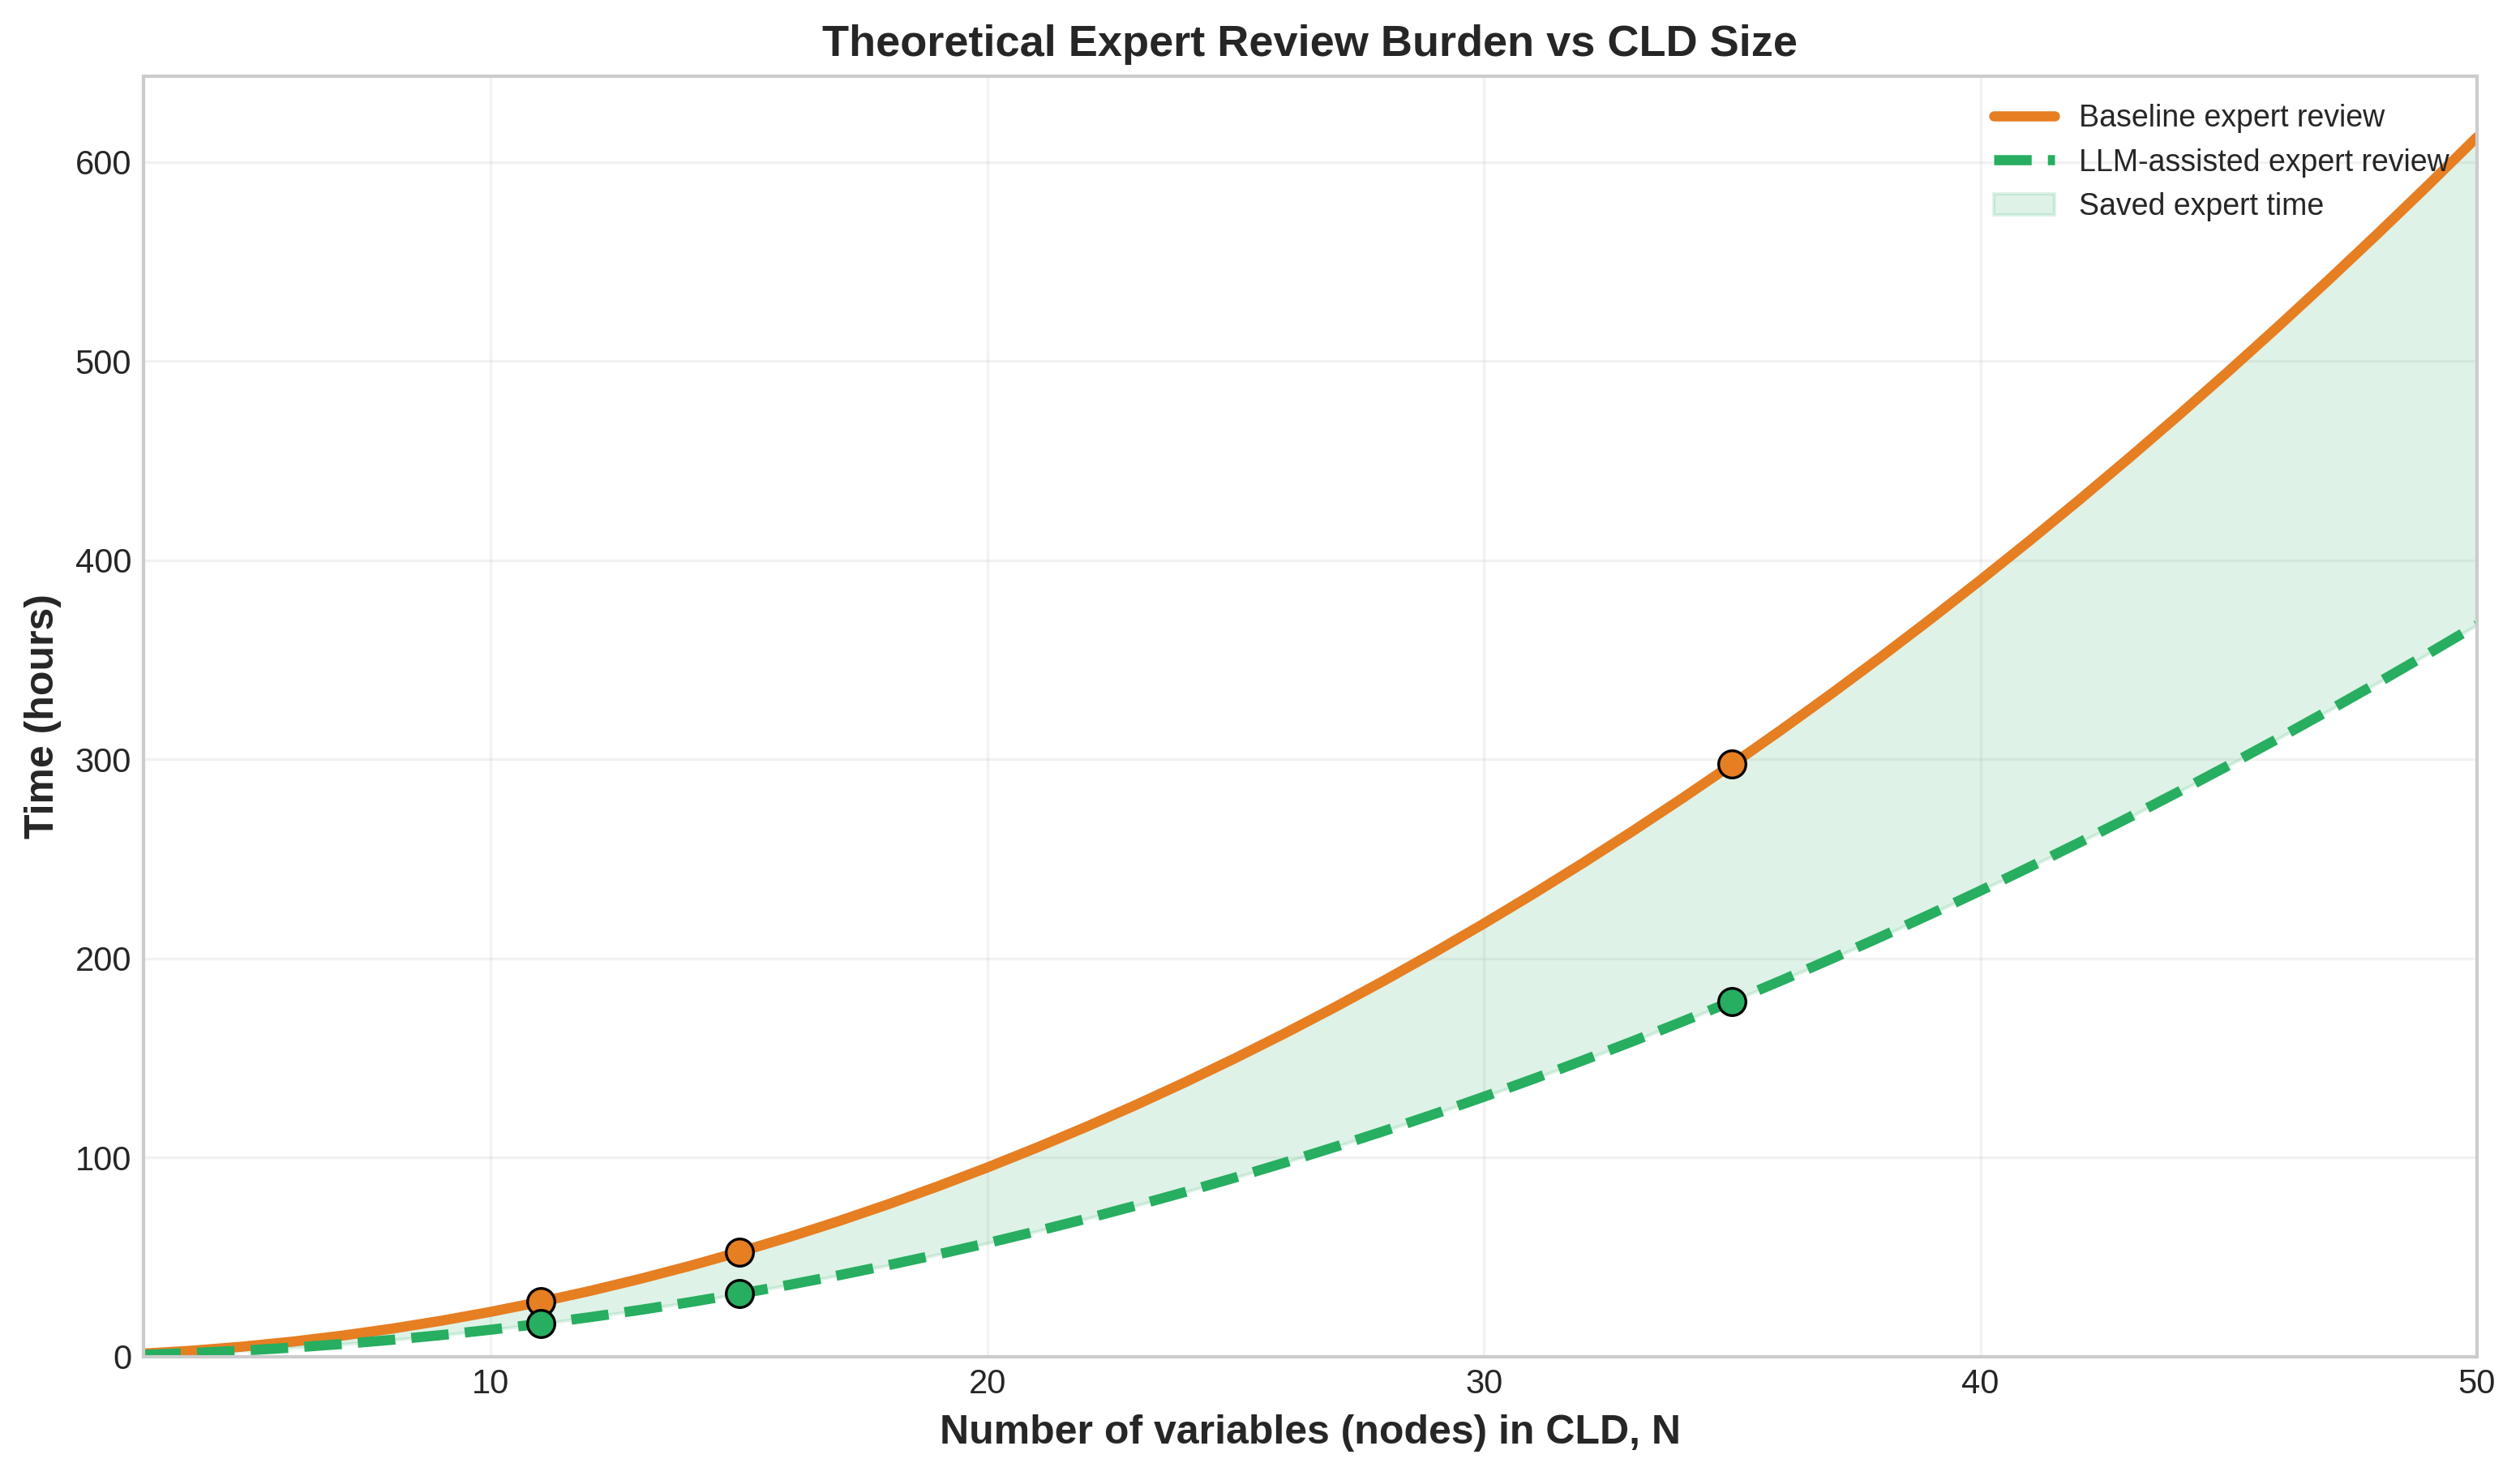
\includegraphics[width=\linewidth]{../../final_runs/time_and_cost_scaling/figures/figure4_expert_time_vs_llm_generation.pdf}
\caption{\textbf{Theoretical expert review burden vs CLD size.} Candidate relationships scale as $O(|V|^2)$. Baseline assumes 5 min/pair across 3 experts. LLM-assisted assumes 50\% valid generation requiring only light validation (1 min/pair); remaining 50\% require full review. Shaded area shows potential time savings.}
\label{fig:expert_review_burden_llm_assisted}
\end{figure}

\medskip
\noindent
\textbf{The hallucination problem.} However, this paradigm shift is contingent on one critical requirement: the LLM must faithfully reproduce relevant information from the literature. LLMs are known to hallucinate---generating plausible-sounding but factually incorrect content---a challenge that persists despite increases in pretraining compute and data scale~\citep{kalai2025languagemodelshallucinate, xu2025hallucination}. If the starting CLD produces spurious connections instead of valid representations of literature findings, the generated CLD will not serve as a useful starting point; it may actively mislead expert deliberation.

Current literature on LLM-based CLD construction focuses primarily on \emph{causal translation}---extracting causal relationships from provided text---which can reduce hallucination through Retrieval-Augmented Generation (RAG). However, this approach assumes availability of a relevant corpus and is fundamentally capped by retrieval quality. An alternative paradigm is \emph{LLM-based CLD generation}, where the model synthesizes causal relationships from its parametric knowledge without requiring an external corpus. This approach is relatively inexpensive and corpus-independent, but suffers from hallucinations that must be detected and mitigated.

Corpus-independent hallucination reduction methods---such as multi-agent LLM-as-a-Judge configurations and low-cost logit-based uncertainty quantification---have shown promise for reducing hallucinations in general LLM applications, but remain untested in the CLD generation context. The critical question---which this thesis addresses---is whether we can detect when LLMs diverge from expert consensus (hallucinate) and whether such divergences can be corrected or validated.

\medskip
\noindent
\textbf{Operationalizing hallucinations and ground truth.} Hallucinations in LLMs manifest as confabulations, inconsistencies, or failures to follow instructions~\citep{ji2023survey, huang2025hallucination}. In the CLD context, we operationalize \emph{hallucinations} as incorrectness in causal links: the erroneous presence (false positive) or absence (false negative) of edges, wrong polarity, or invalid causal reasoning. To evaluate LLM-generated CLDs, we require ground truth---CLDs against which generated outputs can be compared.

This thesis uses two complementary ground truth types. \emph{Literature-derived ground truth} (GT Lit) consists of CLDs published in peer-reviewed literature with explicitly defined causal structures (named variables, directed edges, polarities). A generated edge is classified as a \emph{true positive} if it matches an edge in the literature CLD, a \emph{false positive} (hallucination) if it appears in the generated CLD but not the literature CLD, and a \emph{false negative} if it appears in the literature CLD but was not generated. \emph{Synthetic ground truth} (GT Synth) provides controlled hallucinations by programmatically corrupting valid LLM-generated edges---introducing spurious edges, flipping polarities, or replacing valid causal reasoning with plausible-but-flawed explanations. Here, hallucination status is known by construction (corrupted = hallucination), enabling precise measurement of detection methods under controlled conditions.

This dual operationalization enables quantitative evaluation using standard classification metrics (precision, recall, F1). GT Synth provides controlled conditions for method development, while GT Lit tests generalization to realistic expert-derived ground truth---acknowledging that literature CLDs represent expert-hypothesized relationships rather than empirically validated causal ground truth, a common limitation in complex systems where controlled experiments are infeasible.

\medskip
\noindent
\textbf{Generation: reproduction, synthesis, or new knowledge creation?} Can LLMs perform causal inference? This is a key question, and the answer is not apparent from the properties of the autoregressive language modeling process and the next-token prediction objective~\citep{zecevic2023causalparrots}. The goal of an LLM is to produce the most likely token in a sequence based on its training data. Given this, when prompting an LLM for causal relationships between variables A and B, the model produces an aggregate best guess---the most likely continuation of the sequence given its training data, reflecting patterns learned from related sequences. For reproducing literature consensus or performing synthesis, this may be sufficient, as the LLM has been trained on scientific literature. However, for causal inference in novel settings, LLMs may not be reliable, as they are known to perform worse out-of-distribution~\citep{jin2023cladder, joshi2024causalfallacies}, and estimates of out-of-distribution performance may be overstated as benchmarks enter training datasets through retraining processes. This serves as a note of caution against assuming performance transfers to out-of-distribution settings---a concern amplified by the fact that for many commercial LLMs, the training distribution is unknown, making this impossible to verify.

Furthermore, whether, when, and to what extent LLMs can effectively compress and translate the information reflected in their training data to token space such that it leads to correct answers remains a difficult question. State-of-the-art models exhibit unpredictable failure modes and jagged capability frontiers~\citep{kiciman2024causal}. Established practices exist to identify and mitigate these hallucinations, and this thesis draws from and applies these methods to the CLD generation context.

\medskip
\noindent
\textbf{Beyond reproduction: expert bias mitigation and the possibility of surfacing overlooked relationships.} Crucially, it is possible that not all LLM-generated edges that diverge from expert models are errors. Expert groups operate under time constraints, cognitive biases, and disciplinary blind spots; they may omit relationships due to scope decisions, lack of awareness of adjacent literatures, or simple oversight. This problem intensifies in large-variable systems: for a CLD with $|V|$ variables, considering all pairwise relationships scales as $O(|V|^2)$, making exhaustive deliberation impractical (cf.\ Figure~\ref{fig:expert_review_burden_llm_assisted}). An expert group modeling a 50-variable system faces 2,450 potential edges---far more than can be carefully discussed in a typical workshop.

In such settings, LLM-generated edges not found in expert CLDs may represent plausible causal relationships supported by scientific literature that experts simply did not consider. If validated against the literature, these edges could \emph{augment} expert models rather than corrupt them. If evidence supports LLMs' effectiveness in this manner, it could reframe the LLM's role: not merely as a reproducer of expert consensus, but also as a tool for surfacing relationships the literature supports but experts overlooked. The challenge then becomes distinguishing genuine hallucinations (unsupported fabrications) from overlooked-but-valid relationships---a distinction that motivates the Deep Research validation approach explored in this thesis.

\medskip
\noindent
\textbf{The false negative problem.} Conversely, \emph{false negatives}---relationships that experts include but LLMs omit---represent a distinct challenge. These gaps may arise from several sources: (1) tacit clinical or practical knowledge that experts hold but is underrepresented in published literature; (2) recent findings not yet incorporated into LLM training data; (3) domain-specific terminology that differs from how relationships are described in text; (4) relationships established through unpublished pilot studies, clinical intuition, or cross-disciplinary insights that experts bring to group model building sessions; or (5) LLM reproduction failure---cases where the relationship \emph{is} well-documented in literature but the LLM fails to retrieve or generate it, representing a form of omission-hallucination distinct from fabrication. False negatives are particularly problematic because they represent genuine expert knowledge that LLM-generated drafts would miss, potentially leading to incomplete models if experts do not carefully review and augment the LLM output.

\medskip
\noindent
\textbf{Mitigating hallucinations.} LLM hallucinations---fabricated or inconsistent outputs---undermine reliability for scientific applications~\citep{zhao2023explainability, varshney2023stitch}. A growing body of work has explored both black-box and white-box mitigation strategies. Black-box approaches include prompting techniques such as chain-of-thought reasoning~\citep{wei2022chain, brown2020language}, retrieval-augmented generation~\citep{lewis2020retrieval, zhang2024causal}, multi-agent orchestration and debate~\citep{shinn2024reflexion, lu2024ai}, LLM-as-a-Judge evaluation~\citep{zheng2024judging}, and test-time compute scaling~\citep{openai2024reasoning, shinn2024reflexion, guo2025deepseek}. White-box approaches---which require model weight acess---include fine-tuning~\citep{hu2021lora}, reinforcement learning from human feedback~\citep{ouyang2022rlhf}, and activation monitoring or steering~\citep{wang2024adaptive}. These methods have shown promise for reducing hallucinations across various NLP tasks~\citep{tonmoy2024comprehensive}.

LLM-as-a-Judge (Judge) approaches offer the advantage of context-awareness: they can evaluate outputs against nuanced domain requirements without requiring explicit ground truth, based on the parametric knowledge of the Juging LLM. However, Judges remain vulnerable to biases inherent to transformer architectures and can be susceptible to adversarial manipulation~\citep{li2024llms, shi2024optimization}. Conversely more naive hallucination detection UQ metrics based on generator logprobs or retrieval based approaches ---such as embedding-based similarity~\citep{lewis2020retrieval, zhang2024causal}, perplexity~\citep{valentin2024cost, tonmoy2024comprehensive}, and minimum generation probability~\citep{varshney2023stitch}---provide computationally efficient signals that are robust to contextual manipulation but lack semantic understanding of task requirements. The combination of LLM-as-a-Judge with naive UQ metrics remains under-explored in CLD generation, yet represents a promising approach: UQ metrics could flag high-uncertainty generations for judge evaluation, potentially reducing the biases of judge-only systems while enabling more efficient allocation of test-time compute for self-correction.
This motivates the research questions of this thesis.

%------------------------------------------------------------------------------
\subsection*{Research Questions}
%------------------------------------------------------------------------------

This thesis investigates how LLM-as-a-Judge and UQ metrics can detect and mitigate hallucinations in LLM-generated CLDs, structured around the following research questions:

\begin{description}
    \item[RQ1:] \textbf{Can LLM-as-a-Judge methods detect hallucinations in LLM-generated CLDs?}
    \begin{description}
        \item[RQ1a:] How effectively can correctness-based and citation-based judges distinguish valid from hallucinated causal relationships?
        \item[RQ1b:] Can LLM-as-a-Corrector improve CLD accuracy when guided by judge feedback?
    \end{description}
    
    \item[RQ2:] \textbf{Can uncertainty quantification (UQ) metrics predict hallucinations in generated CLDs?}\\
    Specifically, can logit-derived uncertainty metrics (perplexity, minimum probability, window entropy) and embedding-based similarity detect hallucinated edges?
    
    \item[RQ3:] \textbf{Can smart test-time compute allocation improve CLD accuracy efficiency?}\\
    Can selective deployment of LLM-as-a-Judge \& Corrector---triggered by high uncertainty metrics---provide a more efficient accuracy-per-dollar tradeoff than always-on LLM-as-a-Judge \& Corrector?
\end{description}

%------------------------------------------------------------------------------
\subsection*{Significance and Contributions}
%------------------------------------------------------------------------------

This research addresses reliability challenges in LLM-based scientific knowledge generation by systematically evaluating hallucination detection methods in the CLD domain. The work is timely: as LLM-based systems are increasingly deployed for knowledge work assistance across institutional and global scales, the accuracy of AI-generated outputs carries significant real-world consequences---particularly in health domains where CLDs inform clinical decision-making and intervention design.

Integrating hallucination detection techniques within a CLD-building system is novel and addresses a critical gap: while LLM-as-a-Judge and logit-based uncertainty methods have been studied separately in general NLP contexts, their combined application to structured scientific knowledge generation---specifically causal diagrams---remains unexplored. This thesis makes the following contributions:

\begin{enumerate}
    \item \textbf{Systematic evaluation of LLM-as-a-Judge for CLD validation.} We compare correctness-based and citation-based judges across multiple prompt variants and validation settings. We establish that judges achieve substantial agreement with human experts, but exhibit systematic leniency bias that makes them better suited for screening and triage than definitive validation. Performance transfers only partially from synthetic corruptions to expert-derived ground truth, with effectiveness varying by domain and prompt design.
    
    \item \textbf{Evaluation of LLM-as-a-Corrector for CLD refinement.} We assess whether LLM correctors, conditioned on judge feedback, can improve CLD quality. We find that correctors yield modest gains on synthetic corruptions but fail to improve accuracy against literature-derived expert ground truth. A key finding is that correctors optimize for judge satisfaction rather than expert consensus---judge scores improve while ground truth alignment worsens---revealing a fundamental limitation of judge-guided correction.
    
    \item \textbf{Analysis of generator uncertainty metrics for hallucination detection.} We evaluate whether generation-time signals (logit-derived uncertainty and embedding similarity) can predict hallucinated edges without external retrieval. We find that individual metrics provide weak discriminative signal, and while ensemble classifiers achieve strong in-distribution performance, they exhibit poor cross-domain generalization, limiting their utility as standalone detectors.
    
    \item \textbf{Deep Research validation paradigm.} We pilot automated multi-agent literature search as an alternative to correction-based approaches, shifting from \emph{correction} to \emph{validation}. We find that Deep Research retrieves direct causal evidence for a substantial fraction of edges classified as false positives against expert ground truth, suggesting that expert CLDs may systematically underestimate LLM generation quality and that many apparent ``hallucinations'' (edges not found in literature ground truth CLD's) cuould represent overlooked-but-valid causal relationships in isolation.
    
    \item \textbf{Ground truth enrichment framework.} We develop and evaluate a methodology for enriching expert CLDs with literature-validated LLM-generated edges. Through human validation, we identify causal evidence the Deep Research system finds to be strong and largly applicable to the evaluated causal relationships.
    Including these relationships in the ground truth leads to a subtial improvement in the F1 score of the LLM-generated CLDs, suggesting that the ground truth may be incomplete and that the LLM-generated CLDs may be missing causal relationships under strong assumptions. This reframes the evaluation of LLM-generated CLDs: rather than viewing divergence from expert models as error, validated divergences may represent opportunities for model augmentation.
\end{enumerate}

The practical implication is that LLM-generated CLDs, when validated through the methods evaluated here, can provide literature-grounded starting points for expert model-building sessions. This allows domain experts to focus on contributing specialized knowledge rather than reiterating established consensus, improving the efficiency of the modeling process and resulting in more comprehensive CLDs for translation into computational models for research, clinical applications, and intervention simulations.

%------------------------------------------------------------------------------
\subsection*{Thesis Structure}
%------------------------------------------------------------------------------

\begin{description}[leftmargin=1.5em, labelindent=0em, itemsep=1pt, parsep=1pt]
    \item[Chapter 2 -- Background:] Formalizes CLDs as signed directed graphs, situates them within the modeling-simulation cycle, gives an overview of LLM architecture, used prompting techniques, hallucination issues, and established solutions from other fields.
    \item[Chapter 3 -- Related Work:] Contrasts text-to-CLD versus corpus-independent generation paradigms; surveys LLM-as-a-Judge, logprobs-based uncertainty metrics, and test-time compute strategies in more detail.
    \item[Chapter 4 -- Methods:] Describes ground truth datasets, synthetic hallucination protocol, generator/judge/corrector configurations, logprob-based UQ metrics, embedding-based UQ metrics (both in isolation and combined in ensemble classifiers), and the Deep Research multi-agent validation system. Experimental design, evaluation metrics, baselines, and statistical analysis are also covered.
    \item[Chapter 5 -- Results:] Reports generator baseline comparisons; judge performance on synthetic versus literature ground truth; corrector effects on CLD F1 and judge scores; cross-domain UQ metric generalization failure; ensemble classifier performance; and DR evidence for 62\% of ``hallucinations.''
    \item[Chapter 6 -- Discussion:] Interprets the GT Synth--GT Lit performance gap; identifies judge and corrector failure mechanisms; discusses UQ metric results, the pivot to DR that reframes many FPs as overlooked-but-valid edges; discusses limitations and offers directions for future work and practitioner recommendations.
    \item[Chapter 7 -- Conclusion:] Positions LLM-generated CLDs as expert-refinable drafts rather than final outputs; highlights literature-supported ``hallucinations'' as enrichment opportunities.
\end{description}






